\chapter{Detection of dynamic gestures}

\section{Proposed methods}

The dynamic gesture recognition problem is a problem, where the input data consist of a list of consecutive positions and orientations of hand and fingers. 
Moreover, the important factor for recognition is the time dependencies between sequences of hand and finger positions.
Another challenge comes with the fact, that the gestures performed slower and faster should be recognized as the same dynamic gesture.

The proposed solution utilizes parts of the solution used for recognition of the static gestures.
Each frame of the captured data is described by the feature set similarly to the static solution presented in Chapter~\ref{staticChapter}.
The set of features for each frame is then processed by the Hidden Markov Model scheme. 

\subsection{Hidden Markov Model}

A HMM can be considered a finite, $N$-element set of states (a graph), which are associated with the probability distribution.
A Hidden Markov Model is model of a system with the Markov property.
The Markov property means that the next, future state depends only on the previous state and probability of transition between those states.
The first introduction of HMM comes from the work of L. E. Baum et al. \cite{hmmfirst}, who proposed the mathematical background for HMMs.

The transitions between states are represented by the transition probabilities usually stored in $N \times N$ matrix $T$.
In every state, one of the observation from the finite, $K$-element observation set can be generated with observation probability usually represented by the $N \times K$ emission matrix $E$.
The finite set of all possible observation is called the alphabet.
The HMM also consist of a $N$-element vector of initial state probabilities $\Pi$ of the hidden starting state.
Each HMM can be fully defined by the ($T$, $E$, $\Pi$).

\begin{figure}[htbp!]
\centering
 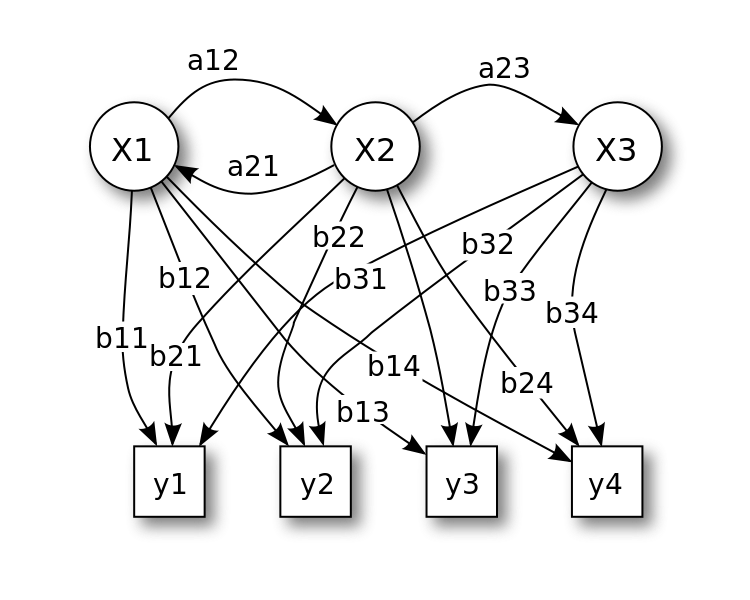
\includegraphics[width=0.8\columnwidth]{figures/HMM_wiki.png}
 \caption[]{Solution blocks of learning and testing parts in task of dynamic gesture recognition\footnotemark}
 \label{dynamicgestureswiki}
\end{figure}

\footnotetext{\url{http://en.wikipedia.org/wiki/File:HiddenMarkovModel.svg}}

The example HMM can be seen in Fig.~\ref{dynamicgestureswiki}.
The HMM in the figure consists of 3 states $\{X1, X2, X3\}$ and 4 possible observations $\{y1, y2, y3, y3\}$.
The probabilities $a_{ij}$ define the transition probability from state $j$-th to state $i$-th. 
The probabilities $b_{ij}$ define the observation probability of generating $j$ observation while being in state $i$.

The HMM can be understood as a directed graph with two types of weighted vertices. 
This way, each state is represented by one type of vertices while observations can be shown as second type of vertices.
There are no edges between vertices representing observations.
The probability values for edges are stored in $T$ and $E$ matrices.

There are three main algorithms used with the HMMs:
\begin{itemize}
\item Forward-Backward algorithm \cite{hmmtutorial, hmm}, 
\item Viterbi algorithm \cite{hmmtutorial, hmm},
\item Baum-Welch algorithm \cite{hmmtutorial, hmm}.
\end{itemize}

The algorithms are shortly described in the following subsections.

\subsection{Forward-Backward Algorithm} 

The Forward-Backward algorithm is used to find the posterior probability of given states given the set of observations.
Given the set of $N$ hidden state variables $X = \{X_1, X_2, ..., X_N\}$ and a sequence of $t$ observations $o_{1:t} = \{o_1, o_2,...,o_t\}$, the algorithm computes probability of state given the observed sequence $P(X_i | o_{1:t})$.
The algorithm utilizes a dynamic programming approach, by performing three steps in a loop: 
\begin{enumerate}
\item computing forward probabilities,
\item computing backward probabilities,
\item computing smoothed values.
\end{enumerate}
The forward pass phase for all states $i=1,..,N$ computes probability $P(X_i | o_{1:k})$, where $k$ is smaller than t, which represent the probability of ending up in state $X_i$ after first k observations. 
The backward pass computes probability $(P(o_{k+1:t}) | X_i)$, which are the probabilities of observing the rest of the observations from the state $X_i$.
The smoothing part uses Bayes rule to compute the probability of state $X_i$ given the whole observation sequence:
\begin{equation}
P(X_k | o_{1:t}) = P(X_k | o_{1:k}, o_{k+1:t}) \propto P(o_{k+1:t} | X_k) P(X_k | o_{1:k}).
\end{equation}
The time complexity of this algorithm is $O(N^2 T)$, where $T$ is the length of observation sequence and $N$ is the number of possible states.


\subsection{Viterbi Algorithm}

The Viterbi algorithm is used to find the most likely sequence of hidden states that best explain the set of observations.
The set of those states is called the Viterbi path. 
The path can be found using the dynamic programming and implementing the equations:
\begin{equation}
\begin{cases} V_{1,k} = P(o_1 | k)  \Pi_k & \mbox{for } k = 1..N \\ V_{t,k} = P(o_t | k)  \argmax_{x\in X} (a_{x,k}  V_{t-1,x}) & \mbox{for } k = 1..N\mbox{ and } t = 2..T \end{cases}
\end{equation}
The solution can be understood as finding a path with maximum probability $\argmax_{x\in X} (V_{T,x})$. 
The time complexity of the algorithm is $O(N^2 T)$, where N is the number of states and T is the observation length and is equal to the complexity of the Forward-Backward algorithm.

\subsection{Baum-Welch Algorithm}

The Baum-Welch algorithm is the algorithm used to find the unknown parameters of the HMM.
For each training example, the algorithms computes the state transition probabilities, observation probabilities in each state and initial probabilities, which maximize the likelihood of observed sequence.
Having the set of sequences of observations, the algorithm can be used to train HMM to detect the sequences similar to the ones used in learning process.
The algorithm uses the results obtained by the Forward-Backward algorithm to iteratively update the probabilities in the emission and the transition matrices.
The training process is stopped after the desired level of a convergence is reached.


\subsection{Structure of the HMM}

\begin{figure}[htb]
\centering
 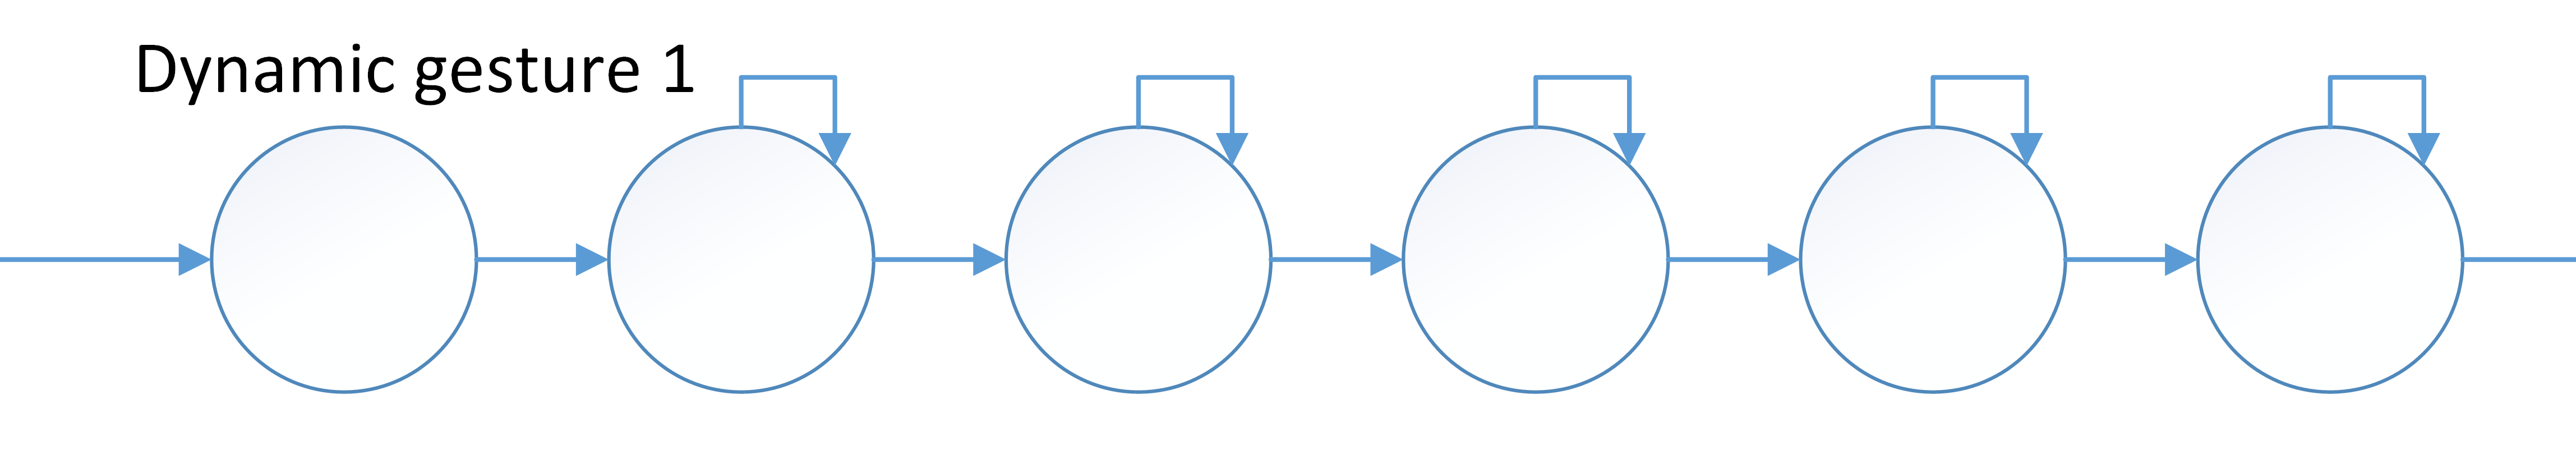
\includegraphics[width=1\columnwidth]{figures/SingleHMM.png}
 \caption{Structure of the HMM's states and non-zero transitions used to detect a single dynamic gesture}
 \label{singlehmm}
\end{figure}

In the dynamic gesture recognition task, we adopted a structure of HMM where each state has non-zero transition probabilities to itself and to the next state in the sequence.
The proposed structure is presented in Fig.~\ref{singlehmm} and was proposed by Yang et al.~\cite{hmm}.
The states can be understood as the phases of hand movement that happen when a wanted gesture is performed.
The self-transitions are used to model the different speeds of the gestures and thus allow to achieve a more robust system.
This structure after training process can be used to measure the probability that the dynamic gesture occurred given the set of observations.

\begin{figure}[htb]
\centering
 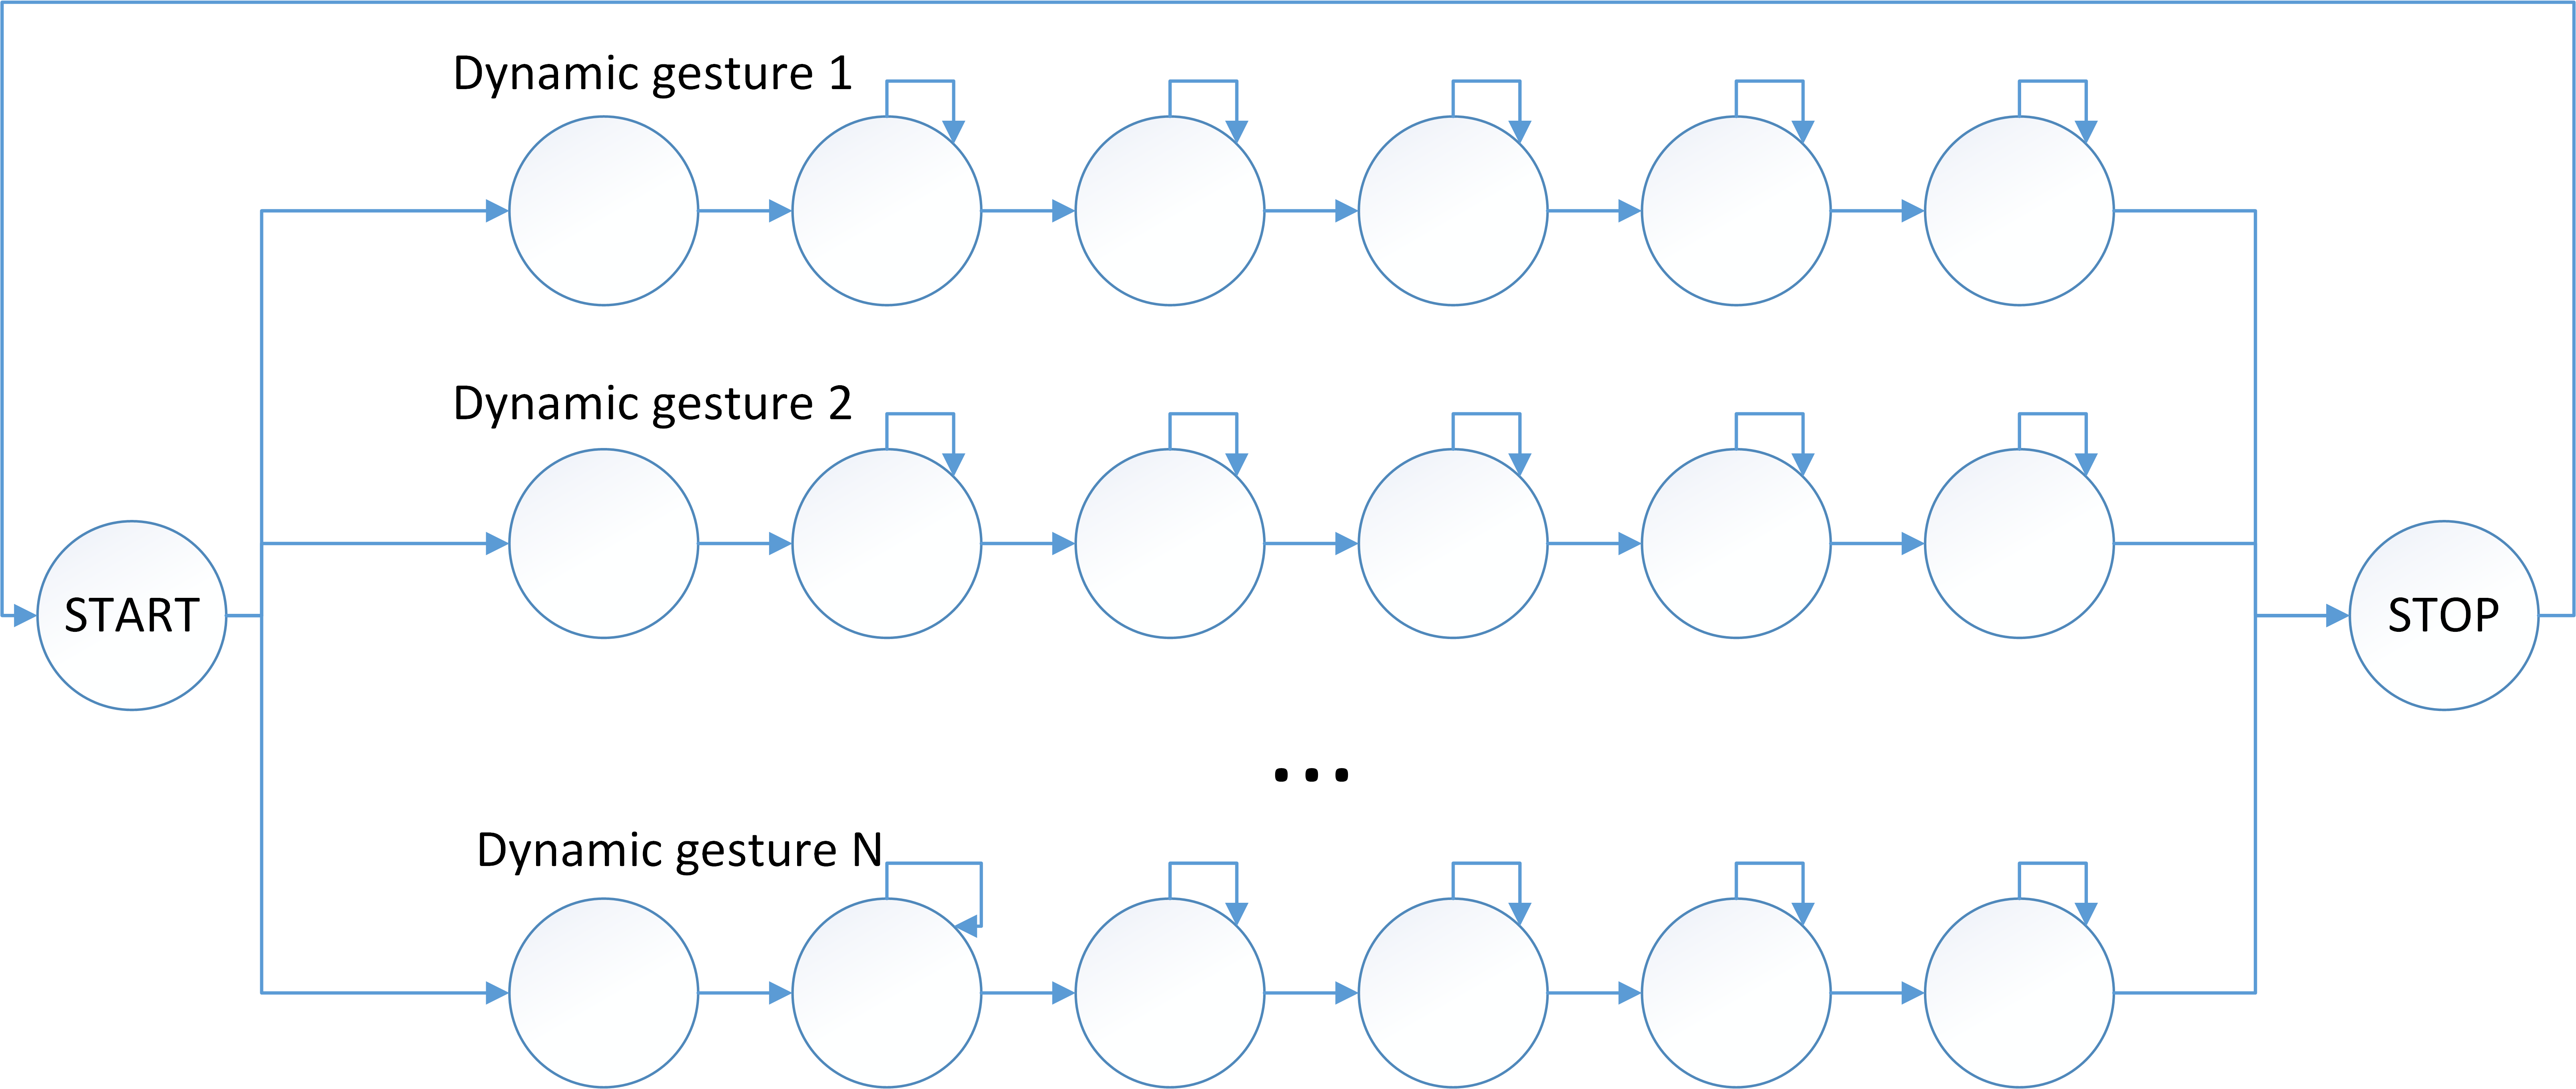
\includegraphics[width=1\columnwidth]{figures/HMM_eng.png}
 \caption{Structure of the HMM's states and non-zero transitions used to simultaneously detect one of $M$ dynamic gestures}
 \label{HMMstructure}
\end{figure}

Having the single dynamic gesture recognition problem modelled as the sequence of $N$ states in which $k$-th state is connected by the edges to the $k$ and $(k+1)$ state and to the all observations.
The problem of distinguishing $M$ gestures translates to the problem of computing probabilities for $M$ sequential graphs.
The problem of finding whether and what dynamic gesture occurred is the problem of finding the probabilities from each of the $M$ HMMs.
Alternatively, the $M$ HMMs can be combined into one HMM were those single HMMs are treated as parallel paths.
The structure of proposed single HMM is presented in Fig.~\ref{HMMstructure}.
In this structure, the recognition process is a process of finding, which of the parallel paths is the most probable.

\subsection{HMM observation from Leap Motion data}

One of the problems when designing the system is a problem of correctly preparing the set of observations from the Leap Motion data.
Most of the proposed solutions in the literature assume that the observations are one-dimensional~\cite{hmmtutorial, hmm}.
This poses a challenge as the raw data from Leap Motion is high-dimensional.
This is the reason, why it is needed to reduce the dimensionality of the observation of the single hand in the predefined moment in time.

To do this, unsupervised clustering algorithms were introduced. 
For this task we examined 3 methods:
\begin{itemize}
\item Chinese whispers \cite{CW1, CW2},
\item Girvan-Newman clustering \cite{Newman},
\item k-means with additional methods to determine the number of clusters. \cite{kmeans1, kmeans2}.
\end{itemize}

\subsubsection{Chinese whipsers}
Chinese whispers algorithm is an efficient randomized graph-clustering algorithm, which is time-linear in the number of edges.
The algorithm was proposed in work by Biemann~\cite{CW1} and thoroughly examined in Natural Language Processing problems. 
The main advantage of the algorithm is the ability to independently determine the number of classes. 
In tests, we used the implementation available in dLib-ml library~\cite{dlib}, which provides multiple implementations of machine learning algorithms.

\subsubsection{Girvan-Newman clustering}
Girvan-Newman clustering is a hierarchical algorithm used to detect clusters in a data represented as a graph.
The algorithm progressively removes edges from the original network until it reaches the maximal number of iterations or an error condition is met.
An adjacency matrix is used to represent the edges between data, where edge value is the similarity between two data points.
The algorithm iteratively calculates the eigenvalues of a created matrix using the power iteration method. 
In case of a complete graph, this algorithm is relatively slow.

\subsubsection{K-means clustering}
Another proposed approach is k-means clustering algorithm.
The idea for the algorithm comes from polish mathematician Hugo Steinhaus, but the first practical application has been presented by MacQueen~\cite{kmeans2}.
The algorithm initially randomly selects $k$ starting points and iteratively performs two steps utilizing the idea of expected-maximization~\cite{expectedmaximization}:
\begin{enumerate}
\item For each data sample the algorithm calculates the distances to $k$ centroids and labels the samples with the label of the centroid with the smallest distance.
\item For each class, the algorithm recalculates centroids position to the averaged position of all samples belonging to class.
\end{enumerate} 
The algorithm stops after the maximum number of iterations or when the change between two consecutive iterations is smaller then defined value.
Unfortunately, the algorithm requires prior knowledge of the number of expected classes.
Nevertheless, there exist heuristics methods aiding in correctly choosing the number of classes. 
One of those methods is plotting the sum of squares error(SSE) within classes against the number of chosen classes. 
The plot is then visually inspected and the fall in error is sough.
The argument for which the drastic error drop is observed is believed to be the correct number of classes in the provided data.

Another, more formal approach introduces the measure of dissimilarity and is called Silhouette width \cite{silhouette}.
Declaring $a(i)$ as the average dissimilarity measure to other samples in the same cluster and $b(i)$ as the lowest average dissimilarity measure to samples in the other clusters which $i$ is not a part of.
The measure of each cluster corrected is proposed to be computed by:
\begin{equation}
s(i) = \frac{b(i) - a(i)}{\max{\{a(i),b(i)}\}}
\end{equation}
The big value of $s(i)$ implies good clustering, while small value of $s(i)$ suggests that the number of classes was not properly chosen.
The $s(i)$ values are used to find the proper number of clusters.


\begin{figure}[htb]
\centering
 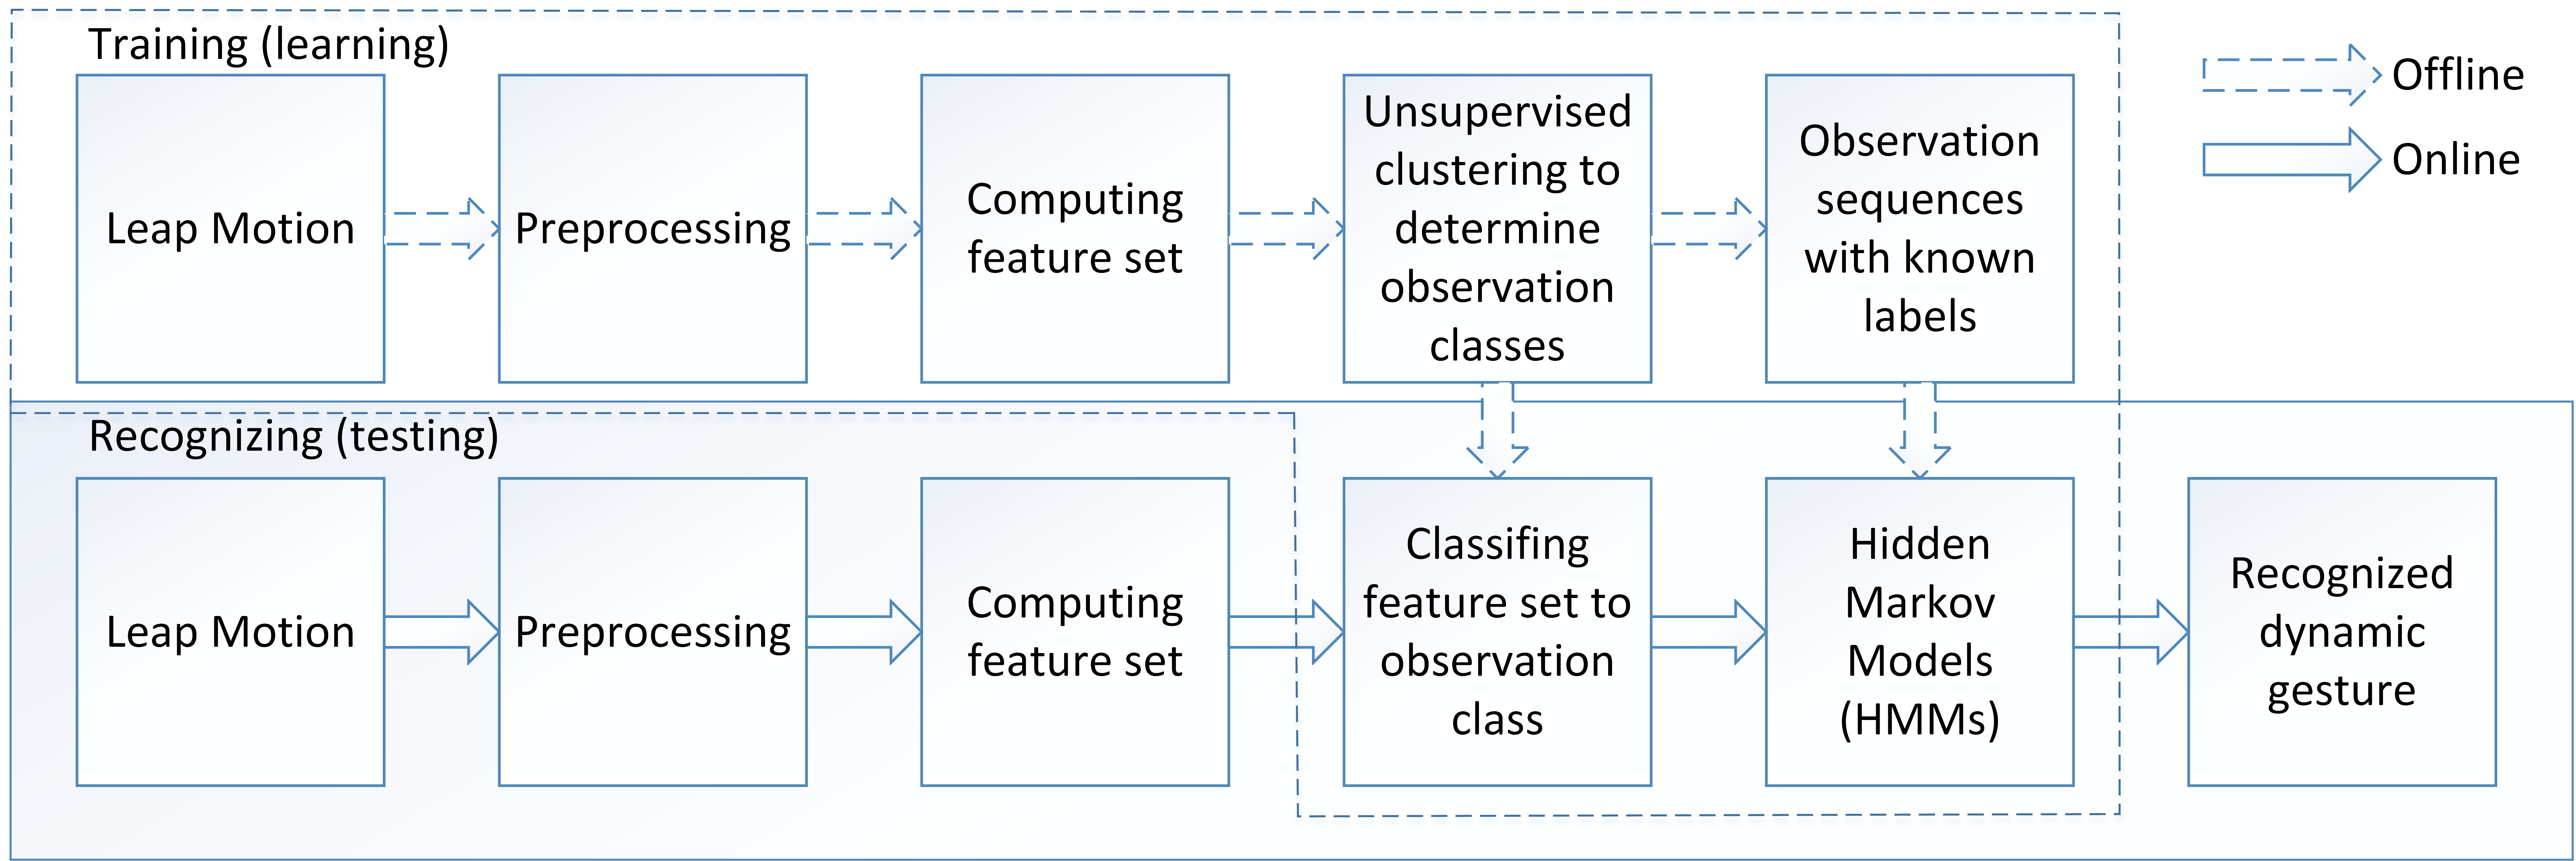
\includegraphics[width=1\columnwidth]{figures/DynamicGestures.png}
 \caption{Solution blocks of learning and testing parts used in the dynamic gesture recognition}
 \label{dynamicgesturesflow}
\end{figure}

\subsection{Whole processing algorithm}
The designed processing algorithm is presented in Fig.~\ref{dynamicgesturesflow}.
The solution consists of two parts: an offline learning and an online recognition.
In learning part, the raw data is preprocessed and then the feature set is extracted. 
Those features are extracted for all recorded positions in training data.
Then one of the unsupervised clustering algorithms is used to find the clusters in the data and then classify those feature sets into observation clusters.
Computed sequences of observation classes represent each dynamic gesture as a series of one-dimensional observations.
For each dynamic gesture, the corresponding HMM is learnt using the Baum-Welch algorithm on the sequence of observations.
The Baum-Welch algorithm computes the matrices that maximizes the probability for one sequence of observations. The problem of training on multiple training data was encountered.
Using the idea presented by Petrushin~\cite{hmmtutorial}, where each matrix trained by one training example is incorporated into hmm's transition matrix using addition with a learning rate $\mu$.
Denoting the transition matrix of HMM by $T$ and learnt transition matrix $T_{new}$, it can be written:
\begin{equation}\label{eq:dynT}
T = (1-\mu) \times T + \mu \times T_{new}.
\end{equation}
The same idea is applied to the emission matrix $E$ and learnt emission matrix $E_{new}$:
\begin{equation}\label{eq:dynE}
E = (1-\mu) \times E + \mu \times E_{new}.
\end{equation}
The learning rate $\mu$ is a value between 0 and 1.
Smaller learning rates results in slower learning, but bigger values may result in no convergence of learning. 
Finding correct learning rate is a task of one of the experiments.
Another problem encountered using this approach is the fact, that matrices no longer represent the probability as the total values in rows do not add to $1.0$.
Therefore, each row of new matrices is normalized to $1.0$.

When dealing with multiple training examples, the learnt solution may adapt to the training samples, but perform poorly on the testing set. 
The problem is known as overfitting to the training samples.
To deal with potential problem, the k-fold cross validation was utilized in a similar approach as in the static gestures presented in Chapter~\ref{staticChapter}.
To complete the training process, each trained HMMs is combined into one recognition structure.

In the recongition, the raw data from Leap Motion is preprocessed, then each frame is labelled accordingly to the classes learnt by the unsupervised clustering algorithm.
The next step includes providing the set of observations to HMMs and running the Viterbi algorithm.
The Viterbi algorithm computes a probability of the the most likely sequence.
Then the maximum probability for each HMM is calculated.
If the maximum probability is above threshold, the gesture is assumed to be correctly recognized with the label of the HMM with the maximum probability sequence.


\section{Evaluation methodology}

To evaluate the quality of recognition achieved by proposed processing pipeline, $6$ dynamic gestures were chosen.
For each of those gestures, we recorded 120 samples (30 samples per each author).
The recorded data contains recordings in different positions with respect to the Leap Motion coordinate system and with different speeds to measure the wanted invariance and robustness of the proposed approach.
The chosen dynamic gestures are:
\begin{enumerate}
\item ``123'' -- counting to three using fingers of one hand,
\item ``door'' -- it's a gesture performed while trying to grasp a handle of a door and then open the door,
\item ``circle'' -- making a circle in the air with the forefinger,
\item ``scissors'' -- simulating cutting an object with scissors made by a forefinger and a middle finger,
\item ``gun'' -- a thumb and an index finger are up with rest of the fingers in a fist. The hand moves up simulating a firing from a gun.
\item ``moving the object'' -- performing the task of grasping an invisible object, moving it and letting it go in a different place.
\end{enumerate}

The $120\times6=720$ samples were divided into training set containing $66,7\%$ of recordings and testing group containing the remaining $240$ recordings. 
The part of the gestures recorded by Katarzyna were used to find the proper number of observation clusters
The training set was used to train each HMM separately on the training data of each gesture.
Preliminary results revealed that initialization of HMM matrices has an impact on the achieved results.
Due to no prior knowledge, the random initialization was chosen.
This approach did not yield reliable solutions in all situation and therefore each training process is performed $10$ times and a model with the best recognition rate from cross-validation is returned.  
Each training cycle of all HMMs takes $1-10$ minutes, with total training part taking $25-60$ minutes.
If not stated otherwise, the learning rate $\mu$ was set to $0.1$, k-cross validation was performed for $k=5$ and the number of states in one HMM was set to $10$.


\section{Experiments}
The experiments are divided into subsections, where in one subsection impact of one parameter is tested.
In first subsection, the number of observation clusters using only the dataset is examined.
The second subsection contains experiments involving different feature sets.
Those subsections are followed by tests involving the impact of number of observation clusters on the total recognition rate of dynamic gestures.
In subsection four, different learning rates are examined. The last subsection presents the impact of the state count on the recognition rate. 

\subsection{Number of observation clusters} \label{numberOfClasses1}

The performed experiments started with testing the unsupervised clustering methods to determine the correct number of observations.
Based on the successful static gesture recognition, each of the hand poses was represented by the vector of values containing:
\begin{itemize}
\item number of detected fingers,
\item $5$ greatest angles between the finger's tip vector and palm normal,
\item $5$ greatest angles between the finger's tip vectors,
\item $5$ greatest distances between the tip positions of fingers.
\end{itemize}
In order to measure a difference between hand poses, the distance function was introduced as the L2 norm between feature vectors for each hand pose:
\begin{equation}
d(x,y) = \sqrt{ \sum_{i=1}^{16} (x_i - y_i)^2 }
\end{equation}
The Chinese whispers and Girven-Newman algorithms use the similarity function $s(x,y)$ which was defined using the difference function $d(x,y)$: 
\begin{equation}
s(x,y) = \frac{1.0}{ \max{\{d(x,y), eps\}}}
\end{equation}
where $eps$ was the numerical epsilon.

For the Chinese Whispers and Girven-Newman clustering the typical parameters from dlib-ml library were used --- the Chinese Whispers maximal iterations were set to $100$, while the Girven-Newman was run with maximal iterations equal to $2000$ and precision epsilon was equal to $1e-4$.
For the SSE analysis the publicly available script was used~\cite{SSE}. 
The script automatically calculates the k-means clustering algorithm for chosen range of $k$ values and presents the figures, which can be a helpful in determining the correct number of classes.
For the Silhouette width analysis R script was written.

\begin{figure}[htbp!]
\centering
 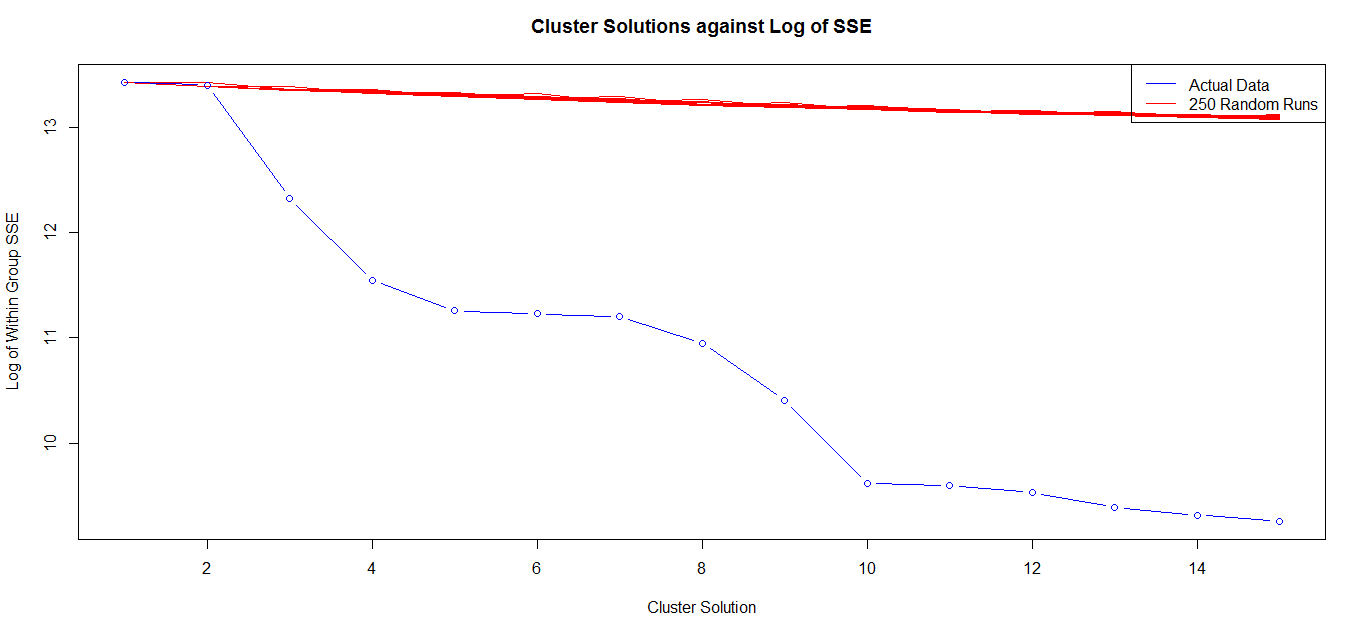
\includegraphics[width=1.0\columnwidth]{figures/SSE1.png}
 \caption{Squared error inside clusters (SEE) as a function of number of clusters for the k-means algorithm}
 \label{dynamicSSE}
\end{figure}

The SSE analysis usually does not yield the direct answer.
The tool provides several plots, but the most interesting one is presented in Fig.~\ref{dynamicSSE}. 
Looking at this plot, there is a significant drop in SSE for the cluster numbers equal to $5$ and $10$.
It is expected that either of those numbers is the correct choice when it comes to the number of classes for k-means algorithm.

\begin{table}[htbp!]
 \caption{Comparison of suggested number of clusters for the dataset containing all positions of hand in all dynamic gesture recordings made by Katarzyna}
 \label{clusterwyn}
    \begin{tabular}{ccccc}
    \hline
     & Girven-Newman & Chinese whispers   & SSE vs clusters & Silhouette width  \\ \hline
    recordings \\by Katarzyna          & -      & $613$ & $5$ or $10$     & $4$     \\ \hline
    \end{tabular}
\end{table}

The Silhouette width approach run on the same data estimated that the there are $4$ distinguishable clusters.
The Girvan-Newman algorithm did not provide any estimate within $24$ hours and therefore was considered impractical.
Chinese whispers algorithm with typical parameters estimated that data contained $613$ clusters.
The proposed values of clusters for different methods are presented in the Table~\ref{clusterwyn}.

Due to the inconclusive results, the analysis of the correct class number was postponed until the correct feature set is chosen.
Until stated otherwise, the class number was assumed to be equal to $10$.

\subsection{Testing different feature sets}
The next challenge was to find the feature set describing one gesture in time, that would contain all necessary information about the dynamic nature of the gesture. 
The first feature set consists of features encoding the information about the speed of the hand. For each $i$-th hand position in recorded sequence, the $(i-10)$-th position was also considered. 
The feature set consisted of the recorded displacement of hand in $X$, $Y$, $Z$ directions.
The number of fingers is also added to feature set containing:
\begin{itemize}
\item a finger count in $i$-th hand position,
\item a finger count in $i-10$-th hand position,
\item a displacement of a hand position in $X$ axis,
\item a displacement of a hand position in $Y$ axis,
\item a displacement of a hand position in $Z$ axis.
\end{itemize}
The presented approach allowed to achieve $64.6\%$ on cross-validation set. 
Due to the small testing set, the total recognition rate was calculated on all available data.
Using all samples recognition rate was equal to $61.8\%$, which is too small to by used in real applications.

The analysis revealed that previous approach suffered from the fact, that the encoded speeds are represented in the coordinate system of the Leap Motion.
Executing the gesture with different angle to the Leap Motion's coordinate system makes the feature set completely different and sometimes results in mislabelling.
Therefore, the feature set was supposed to encode the information with respect to the local coordinate system of hand. 
In new approach, a magnitude of the displacement is calculated. 
It is independent of the chosen orientation of the coordinate system.
To represent the direction of movement, the normalized displacement vector is computed as a vector connecting the center of $i-10$-th hand position with $i$-th hand position.
Then, the dot product between normalized displacement vector and palm normal in $i-10$ position is calculated.
A dot product between the normalized displacement vector and the palm direction is also computed.
The resulting feature contains:
\begin{itemize}
\item a finger count in $i$-th hand position,
\item a finger count in $i-10$-th hand position,
\item a magnitude of the hand's displacement,
\item a dot product of the normalized displacement vector and the palm's normal in $i-10$-th position,
\item a dot product of the normalized displacement vector and the palm's direction in $i-10$-th position.
\end{itemize}
This approach allowed to improve the recognition rate to $69.6\%$ in a cross-validation and to $67.5\%$ on the whole set, but was still not satisfying from the practical point of view.

From the observation of changes in the feature set values on the recorded gestures, it was concluded that sometimes only the fingers are changing positions, while position of hand is steady.
The previous approaches, did not encode this information in feature vectors, which made those changes invisible to the further processing part.
Therefore, the new feature vector contains also the information about the displacement of each corresponding finger.
In order to keep the feature size small, it was decided to only incorporate the magnitude of those displacements. 
Due to the nature of Leap Motion's erratic numbering of fingers, those magnitudes were also sorted.
The total of 4 top values were added to feature vector resulting in feature set:
\begin{itemize}
\item a finger count in $i$-th hand position,
\item a finger count in $i-10$-th hand position,
\item a magnitude of the hand's displacement,
\item a dot product of the normalized displacement vector and the palm's normal in $i-10$-th position,
\item a dot product of the normalized displacement vector and the palm's direction in $i-10$-th position,
\item $4$ greatest magnitudes of finger displacements.
\end{itemize}
The obtained results were even worse than the ones achieved for the feature set two --- $66.1\%$ compared to the previously achieved $67.5\%$ on the whole dataset. 
The further inspection revealed that, while adding displacement of fingers helps in most situations, it can also pose a great risk.
Leap Motion sensor can sometimes change the finger numbering resulting in the displacements calculated between different fingers.
This leads to a big, artificial, phantom displacement.
Therefore, the idea of using a displacement of fingers was abandoned.
 
Looking at the recorded gestures, it seemed that speed information is not sufficient to correctly detect the sequences of gestures combining in one dynamic gesture.
The new feature set contains also the information about the static hand positions allowing to distinguish between dynamic gestures that are comprised of sequential static gestures.
The new feature set contained the already proposed speed part with additional static encoding that was successfully used in static gesture recognition:
\begin{itemize}
\item a finger count in $i$-th hand position,
\item a finger count in $i-10$-th hand position,
\item a magnitude of the hand's displacement,
\item a dot product of the normalized displacement vector and the palm's normal in $i-10$-th position,
\item a dot product of the normalized displacement vector and the palm's direction in $i-10$-th position,
\item the $4$ greatest euclidean distances between all combination of finger's tips in $i$-th position,
\item the $4$ greatest absolute angles between all combination of finger's vectors in $i$-th position,
\item the $4$ greatest euclidean distances between finger's tips and palm's position in $i$-th position,
\item the $4$ greatest absolute angles between finger's vectors and palm's normal in $i$-th position.
\end{itemize}

The experiments showed that the proposed approach allowed to improve recognition rate.
On the other hand, it was believed that the sophisticated static part of feature set is dominating the dynamic part of the feature set, which prevents the method from achieving better results.
Therefore, the $5$-th proposed feature set consists of static part represented only by the $4$ greatest euclidean distances between all combination of finger's tips in $i$-th position and the $4$ greatest absolute angles between all combination of finger's vectors in $i$-th position.
Similarly, feature sets $6$, $7$, $8$ were also the propositions containing the reduced encoding of the static parts, but did not improve significantly over already received results. 
The results obtained by all proposed feature sets are presented in Table~\ref{tab:dyn1}. 

\begin{table}[htbp!]
\begin{center}
	\label{tab:dyn1}
	\caption{Results obtained by the HMM approach using different feature sets}
    \begin{tabular}{|c|c|c|}
    \hline
    ~                                 & $5$ gestures, CV & $5$ gestures, whole dataset  \\ \hline
    feature set $1$                     & $64.6\%$ & $61.8\%$   \\ \hline
    feature set $2$                     & $69.6\%$ & $67.5\%$   \\ \hline
    feature set $3$                     & $68.5\%$ & $66.1\%$   \\ \hline
    feature set $4$          		  & $77.9\%$ & $76.1\%$   \\ \hline
    feature set $5$                     & $66.7\%$ & $63.9\%$   \\ \hline
    feature set $6$                    & $72.9\%$ & $70.4\%$   \\ \hline
    feature set $7$                    & $71.9\%$ & $69.2\%$   \\ \hline
    feature set $8$                    & $78.1\%$ & $77.2\%$   \\ \hline
    \end{tabular}
\end{center}
\end{table}
  
The best results were obtained for feature set $8$, but the results obtained by the full static representation (feature set $4$) are not significantly worse.
For further assessment, the feature set $4$ was chosen as the one that describes each gesture with more information and therefore is believed to work better for gestures that were not included in the experiments.

\subsection{Testing number of observation classes} 

The next experiments were performed to test what is the best number of observation classes for k-means algorithm. 
Previous tests to find the correct number of clusters were performed in Subsection~\ref{numberOfClasses1}, but yield inconclusive results.
Therefore, the tests were performed using the processing algorithm to impact of number of classes on the total recognition rate.
The tests were conducted using feature set $4$ and learning rate $\mu=0.05$.

\begin{table}[htbp!]
\begin{center}
	\label{tab:dynNumber}
	\caption{Results obtained by the HMM approach using feature set $4$ and different numbers of class clusters}
    \begin{tabular}{|c|c|c|}
    \hline
    ~                                 & $5$ gestures, CV & $5$ gestures, whole dataset  \\ \hline
	$k = 4$                  	  & $77.3\%$ & $74.7\%$   \\ \hline
    $k = 5$               	  & $79.6\%$ & $77.6\%$   \\ \hline
    $k = 6$                    & $79.6\%$ & $77.6\%$   \\ \hline
    $k = 8$                     & $77.7\%$ & $76.0\%$   \\ \hline
    $k = 10$                    & $77.9\%$ & $76.1\%$   \\ \hline
    $k = 12$                    & $78.5\%$ & $77.4\%$   \\ \hline
    \end{tabular}
\end{center}
\end{table}
The results are presented in Table~\ref{tab:dynNumber}.
The best obtained results are for the number of clusters $k=5$ and $k=6$ for which an increase in the recognition rate when compared to the previously achieved results. 
The recognition rate in cross-validation was equal to $79.6\%$ and $77.6\%$ on the whole dataset. 

\subsection{Testing learning rate}

The next experiments involved finding the best learning rate. 
Using predefined learning rate may be dangerous as small value may mean small convergence, while too big step may result in not converging to the locally best solution. 
In our application, the stable learning rate through whole training process was chosen to minimize the number of parameters. 
The further developments may involve using learning rate that is changing depending on the already training error.
The experiments were conducted on the same dataset using feature set four, five observation classes and learning rates:
\begin{itemize}
\item $\mu$ = 0.01
\item $\mu$ = 0.05
\item $\mu$ = 0.1
\item $\mu$ = 0.2
\end{itemize}
The achieved results are presented in Table~\ref{tab:dyn2}.
In proposed application, the learning rate $\mu = 0.05$ allowed to achieve the best results and is recommended by the authors of this thesis. 

\begin{table}[htbp!]
\begin{center}
	\label{tab:dyn2}
	\caption{Results obtained by the HMM approach using feature set $4$, $5$ observation classes and different learning rates}
    \begin{tabular}{|c|c|c|}
    \hline
    ~                                 & $5$ gestures, CV & $5$ gestures, whole dataset  \\ \hline
	$\mu$ = 0.01                  	  & $77.5\%$ & $76.9\%$   \\ \hline
    $\mu$ = 0.05                      & $80.4\%$ & $79.0\%$   \\ \hline
    $\mu$ = 0.1                      & $79.6\%$ & $77.6\%$   \\ \hline
    $\mu$ = 0.2                      & $69.6\%$ & $69.7\%$   \\ \hline
    \end{tabular}
\end{center}
\end{table}

\subsection{Testing number of states in HMM}

The only parameter not tested in the already described experiments is the number of state each HMM is composed of. 
The previously used value was equal to $10$ states. 
In the experiments four different values were tested: 5, 10, 20 and 30.
The results from experiments are presented in Tab.~\ref{tab:dyn3}. 
The performed experiments confirmed that smaller number of states ($5$) results in lower recognition rate as the HMM is not complicated enough.
Additionally, number of states greater than 10 did not improve the result.
When choosing the number of states, it is also important to remember about the complexity of algorithms, which are grow quadratically with the number of states, which affects the learning and recognition times. 
The performed experiments and theoretical computational complexity confirm that the computational complexity grows quadratically with the chosen number of states.


\begin{table}[htbp!]
\begin{center}
	\label{tab:dyn3}
	\caption{Results obtained by the HMM approach using feature set $4$, $6$ observation classes and different state elements}
    \begin{tabular}{|c|c|c|}
    \hline
    ~                                 & $5$ gestures, CV & $5$ gestures, whole dataset  \\ \hline
	$K = 5$                  	  & $74.0\%$ & $73.6\%$   \\ \hline
    $K = 10$                     & $79.6\%$ & $77.6\%$   \\ \hline
    $K = 20$                    & $77.5\%$ & $76.5\%$   \\ \hline
    $K = 30$                     & $77.9\%$ & $76.3\%$   \\ \hline
    \end{tabular}
\end{center}
\end{table}